\section{Описание практической части}
\label{sec:Chapter4} \index{Chapter4}

Компилятор рассматриваемого языка в основном написан на языке программирования C++.

Для наглядности далее в тексте в качестве базового примера будут использоваться типы:
int (примитивный) → Int (объектный аналог)

\subsection{Арифметические операции}
На данном этапе работы было необходимо модифицировать проверку корректности типов в арифметческих операциях:
\begin{itemize}[label={}]
    \item \code{+} , \code{-} , \code{+=} , \code{-=}
    \item \code{++} , \code{--}
    \item \code{*} , \code{/} , \code{\%} , \code{*=}, \code{/=}, \code{\%=}
    \item \code{$\langle \langle$} , \code{$\rangle \rangle$} , \code{$\langle \langle$=} , \code{$\rangle \rangle$=}, \code{$\rangle \rangle \rangle$}, \code{$\rangle \rangle \rangle$=}
    \item \code{|} , \code{|=} , \code{\&} , \code{\&=}, \code{\^}, \code{\^}\code{=}, \code{||} , \code{\&\&}
    \item \code{<} , \code{<=} , \code{>}, \code{>=}, \code{==}, \code{===}, \code{!}
\end{itemize}

В существующей реализации почти в каждой функции проверки производилось безусловное приведение типов операторов к примитивным, поэтому первым этапом работы было удаление или изменение кода, который приводил бы к замене объектных типов на их примитивные аналоги. Далее, основная функция, которая была нужна почти для всех вышеперечисленных операций(исключая логические и унарные) - функция, вычисляющая тип результата бинарного выражения. Ее поведение основывается на иерархии численных типов, оговоренной в спецификации.
Следующий этап заключался в очистке кода от попыток свернуть константы в функциях проверки, чтобы вынести все константные вычисления в отдельный модуль.

\subsection{Преобразования типов}
Для реализации проверки легальности преобразования объектных примитивоподобных типов можно было переиспользовать алгоритм, использовавшийся для проверки преобразований примитивных типов, добавив дополнительные проверки на отношения объектов (Union и Enum).
Структура функции для проверки корректности преобразования представлена на \ref{fig:cmp}
\begin{figure}[H]
    \centering
    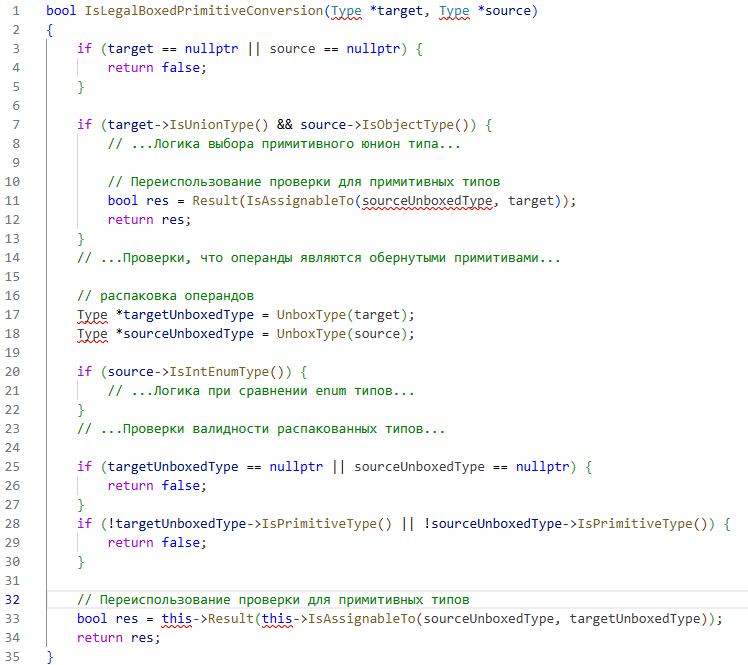
\includegraphics[scale=0.6]{image.png}
    \caption{Структура функции для проверки корректности преобразования примитивоподобных объектов}
    \label{fig:cmp}
\end{figure}

\subsection{Свёртка констант}
Один из основных этапов работы - это имплементация модуля компиляции для сверки констант в начало стадии семантического анализа.
Свёртка констант - вычисление константных выражений с последующей заменой выражений на результаты,
выполняемое на отдельной стадии компиляции. Это оптимизация, которая:
\begin{itemize}[label={--}]
    \item Ускоряет выполнение программы (избегает вычислений в runtime)
    \item Уменьшает размер генерируемого кода
    \item Позволяет обнаружить ошибки на этапе компиляции
\end{itemize}

Исплементированный модуль позволяет рекурсивно обойти const и readonly декларации и заменить константные выражения результатом их вычисления.
\subsubsection{Основной алгоритм}
\begin{enumerate}[label={--}]
    \item \textbf{Обход AST} - рекурсивных обход синтаксического дерева программы
    \item \textbf{Идентификация константных выражений} - проверка, можно ли вычислить выражение на этапе компиляции (является ли выражение константным)
    \item \textbf{Вычисление констант} - выполнение операций над константами
    \item \textbf{Замена выражений} - подстановка вычисленных значений вместо исходных выражений
\end{enumerate}

\subsubsection{Поддерживаемые типы и операции}
\textbf{Типы данных}
\begin{itemize}[label={--}]
    \item Числовые литералы (int, float, double)
    \item Символьные литералы (char)
    \item Булевы значения (true/false)
    \item Строковые литералы
    \item Enum значения
\end{itemize}

\textbf{Операции}
\begin{itemize}[label={--}]
    \item Арифметические  +, -, *, /, \%
    \item Битовые  \&, |, \^{}, \~{}, \verb|<<|, \verb|>>|, \verb|>>>|
    \item Логические  \&\&, ||, !
    \item Сравнения  ==, !=, <, >, <=, >=
    \item Унарные  +, -, \~{}
\end{itemize}

\subsubsection{Детали реализации}
\subsubsection*{Типизация и преобразование типов}
\begin{itemize}[label={--}]
    \item Используется система рангов типов TypeRank для определения приоритета преобразований
    \item Реализованы безопасные преобразования между типами с проверкой диапазонов
    \item Обработка деления на ноль
\end{itemize}

\begin{lstlisting}[language=C++,caption=Перечисление рангов типов]
enum class TypeRank {
    INT8,
    INT16,
    INT32,
    INT64,
    FLOAT,
    DOUBLE,
    CHAR
};
\end{lstlisting}

\subsubsection{Основные функции}
\begin{lstlisting}[language=C++,caption=GetTypeRank]
static TypeRank GetTypeRank(const ir::Literal* lit) {
    if (lit->IsCharLiteral()) {
        return TypeRank::CHAR;
    }

    auto num = lit->AsNumberLiteral()->Number();
    if (num.IsByte()) return TypeRank::INT8;
    if (num.IsShort()) return TypeRank::INT16;
    if (num.IsInt()) return TypeRank::INT32;
    if (num.IsLong()) return TypeRank::INT64;
    if (num.IsFloat()) return TypeRank::FLOAT;
    if (num.IsDouble()) return TypeRank::DOUBLE;

    ES2PANDA_UNREACHABLE();
}
\end{lstlisting}

\textbf{Получение значения литерала}
\begin{lstlisting}[language=C++,caption=GetVal]
template <typename TargetType>
static TargetType GetVal(const ir::Literal* node) {
    // Обработка булевых литералов
    if constexpr (std::is_same_v<TargetType, bool>) {
        return node->AsBooleanLiteral()->Value();
    }

    // Обработка символьных литералов
    if constexpr (std::is_same_v<TargetType, char16_t>) {
        return node->AsCharLiteral()->Char();
    }

    auto numNode = node->AsNumberLiteral();

    // Обработка числовых литералов разных типов
    if constexpr (std::is_same_v<TargetType, int8_t>) {
        return numNode->Number().GetByte();
    }
    if constexpr (std::is_same_v<TargetType, int16_t>) {
        return numNode->Number().GetShort();
    }
    // ...
    if constexpr (std::is_same_v<TargetType, double>) {
        return numNode->Number().GetDouble();
    }
}
\end{lstlisting}

\textbf{Преобразование значений между типами}
\begin{lstlisting}[language=C++,caption=CastValTo]
template <typename To>
static To CastValTo(const ir::Literal* lit) {
    // Обработка булевых литералов
    if (lit->IsBooleanLiteral()) {
        return static_cast<To>(GetVal<bool>(lit));
    }

    // Определение ранга типа и преобразование
    auto rank = GetTypeRank(lit);
    switch (rank) {
        case TypeRank::DOUBLE:
            return static_cast<To>(GetVal<double>(lit));
        case TypeRank::FLOAT:
            return static_cast<To>(GetVal<float>(lit));
        // ...
        case TypeRank::CHAR:
            return static_cast<To>(GetVal<char16_t>(lit));
    }

    ES2PANDA_UNREACHABLE();
}
\end{lstlisting}


\subsubsection*{Обработка ошибок}
\begin{itemize}[label={--}]
    \item Генерация диагностических сообщений для недопустимых операций
    \item Реализованы безопасные преобразования между типами с проверкой диапазонов
    \item Отдельные функции преобразований между целыми и вещественными типами
\end{itemize}

\subsubsection*{Оптимизации}
\begin{itemize}[label={--}]
    \item Использование битовых операций для безопасной работы с целыми числами
    \item Специальная обработка строковых конкатенаций
    \item Оптимизация шаблонных литералов
\end{itemize}

\subsection{Оптимизация}


Реализованная оптимизация представляет собой систему преобразования типов, которая рекурсивно анализирует и модифицирует абстрактное синтаксическое дерево (AST) для выполнения операций nboxing (распаковки) и boxing (упаковки) типов.

\subsection*{Архитектура оптимизации}

\subsubsection{Класс UnboxVisitor}
Рекурсивный анализ дерева проводится с помощью специального класса \texttt{UnboxVisitor}, реализующего методы \texttt{VisitX} для различных типов узлов AST. Его задачи:
\begin{enumerate}
    \item Обойти AST и найти места, где можно заменить boxed-типы на примитивы
    \item Вставить явные преобразования (например, вызовы \texttt{unboxed()}, \texttt{valueOf()}, intrinsic-функции)
    \item Обновить соответствующие типы в выражениях, объявлениях и сигнатурах
    \item Заново запустить функцию валидации ноды
\end{enumerate}


\subsubsection{Обрабатываемые узлы AST}
Примеры обрабатываемых узлов:
\begin{itemize}
    \item \texttt{VisitCallExpression} — вызовы функций
    \item \texttt{VisitBinaryExpression} — бинарные операции (+, ==, \&\& и т. д.)
    \item \texttt{VisitMemberExpression} — доступ к полям/методам (\texttt{obj.field}, \texttt{arr[index]})
    \item \texttt{VisitReturnStatement} — возвращаемые значения
    \item \texttt{VisitVariableDeclarator} — объявления переменных
\end{itemize}

\subsubsection{Механизм работы Visitor'ов}

Каждый узел AST имеет метод \texttt{Accept(visitor)}.
При вызове \texttt{astNode->Accept(visitor)} управление передаётся в соответствующий метод \texttt{VisitX} у UnboxVisitor.

\subsubsection{Пример обработки CallExpression}
\begin{lstlisting}[language=C++,caption=Обработка вызовов функций]
void VisitCallExpression(ir::CallExpression *call) override {
    // 1. Обновление типов аргументов
    for (size_t i = 0; i < call->Arguments().size(); i++) {
        auto *arg = call->Arguments()[i];
        auto *expectedType = call->Signature()->Params()[i]->TsType();
        call->Arguments()[i] = AdjustType(uctx_, arg, expectedType);
    }

    // 2. Обновление возвращаемого типа
    if (call->Signature()->ReturnType()->IsETSPrimitiveType()) {
        call->SetTsType(call->Signature()->ReturnType());
    }
}
\end{lstlisting}

\subsubsection{Логика преобразования типов}
Решение о том, нужно ли вставлять boxing, unboxing или конверсию примитивов, принимается с помощью метода AdjustType:
\begin{lstlisting}[language=C++,caption=Метод AdjustType]
static ir::Expression *AdjustType(UnboxContext *uctx,
                                ir::Expression *expr,
                                checker::Type *expectedType) {
    // Если выражение — примитив, а ожидается объект → boxing
    if (expr->TsType()->IsETSPrimitiveType()
        && expectedType->IsETSObjectType()) {
        return InsertBoxing(uctx, expr);
    }
    // Если выражение — boxed-объект, а нужен примитив → unboxing
    if (TypeIsBoxedPrimitive(expr->TsType())
        && expectedType->IsETSPrimitiveType()) {
        return InsertUnboxing(uctx, expr);
    }
    // Если оба примитива, но разных типов → конверсия
    if (expr->TsType()->IsETSPrimitiveType()
        && expectedType->IsETSPrimitiveType()) {
        return InsertPrimitiveConversion(uctx, expr, expectedType);
    }
    return expr;
}
\end{lstlisting}

\subsubsection{Пример преобразования}

\textbf{Исходный код}
\begin{lstlisting}[language=TypeScript]
let x: Int = 10;  // Int — объектный тип
let y: int = x + 5;   // int — примитив
\end{lstlisting}

\textbf{Преобразование AST}
\begin{lstlisting}[caption=AST до оптимизации]
BinaryExpression(
    left: Identifier("x", type=Int),
    op: +,
    right: NumberLiteral(5, type=int)
)
\end{lstlisting}


\begin{lstlisting}[caption=AST после оптимизации]
    BinaryExpression(
        left: CallExpression(
            callee: MemberExpression(
                object: Identifier("x", type=Int),
                property: "unboxed"
            ),
            type=int
        ),
        op: +,
        right: NumberLiteral(5, type=int)
    )
\end{lstlisting}


\newpage